\documentclass[UTF8]{article}

% % !TeX program = xelatex 
% \documentclass{standalone}
\usepackage{xeCJK}
\usepackage{tikz}
\usetikzlibrary{shapes,arrows}
\usetikzlibrary{fit,calc,positioning,through,hobby}
\usetikzlibrary{decorations.pathreplacing,decorations.markings,through,hobby}

\tikzset{
  % style to apply some styles to each segment of a path
  on each segment/.style={
    decorate,
    decoration={
      show path construction,
      moveto code={},
      lineto code={
        \path [#1]
        (\tikzinputsegmentfirst) -- (\tikzinputsegmentlast);
      },
      curveto code={
        \path [#1] (\tikzinputsegmentfirst)
        .. controls
        (\tikzinputsegmentsupporta) and (\tikzinputsegmentsupportb)
        ..
        (\tikzinputsegmentlast);
      },
      closepath code={
        \path [#1]
        (\tikzinputsegmentfirst) -- (\tikzinputsegmentlast);
      },
    },
  },
  % style to add an arrow in the middle of a path
  mid arrow/.style={postaction={decorate,decoration={
        markings,
        mark=at position .5 with {\arrow[#1]{stealth}}
      }}},
}

\tikzstyle{startstop} = [draw=white,thick]
\tikzstyle{tranfun} = [rectangle,minimum width=0.5cm,minimum height=0.5cm,align=center, draw=black,thick]
\tikzstyle{cmppoi} = [circle,minimum width=1pt,minimum height=1pt,draw=black,thick]

\begin{document}

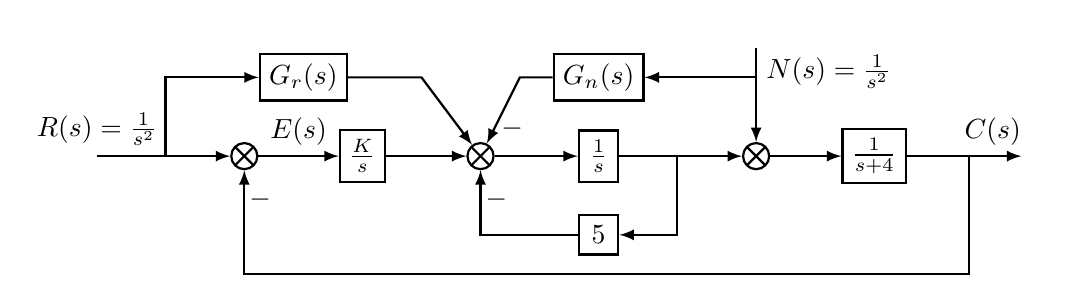
\begin{tikzpicture}[->,use Hobby shortcut,>=latex,thick,node distance = 1.5cm]

\node (start0) [startstop] {};
\node (cmp1) [cmppoi,right of=start0,xshift=0.5cm] {};
\node (tf1) [tranfun,right of=cmp1,xshift=0cm] {$\frac{K}{s}$};
\node (cmp2) [cmppoi,right of=tf1] {};
\node (tf2) [tranfun,right of=cmp2,xshift=0cm] {$\frac{1}{s}$};
\node (cmp3) [cmppoi,right of=tf2,xshift=0.5cm] {};
\node (tf3) [tranfun,right of=cmp3,xshift=0cm] {$\frac{1}{s+4}$};
\node (end0) [startstop,right of=tf3,xshift=0.5cm] {};
\node (tf4) [tranfun,above of=cmp1,shift={(0.75,-0.5)}] {$G_r(s)$};
\node (tf5) [tranfun,above of=tf2,shift={(0,-0.5)}] {$G_n(s)$};
\node (tf6) [tranfun,below of=tf2,shift={(0,0.5)}] {$5$};
\node (start1) [startstop,above of=cmp3] {};

\foreach \x in {-0.11,0.11}
{
	\foreach \y in {-0.11,0.11}
	{
		\foreach \i in {1,2,3}
		{
			\draw[-] (cmp\i.center)--+(\x,\y);
		}
	}
}

\draw (start0)--node[above,pos=0]{$R(s)=\frac{1}{s^2}$}(cmp1);
\draw (cmp1)--node[above]{$E(s)$}(tf1);
\draw (tf1)--node[above]{$$}(cmp2);
\draw (cmp2)--node[above]{$$}(tf2);
\draw (tf2)--node[above]{$$}(cmp3);
\draw (cmp3)--node[above]{$$}(tf3);
\draw (tf3)--node[above,pos=0.75]{$C(s)$}(end0);
\draw ($(start0)+(1,0)$)|-(tf4);
\draw (tf4)--+(1.5,0)--(cmp2);
\draw ($(tf2)+(1,0)$)|-(tf6);
\draw (tf6)-|(cmp2)node[below,shift={(0.2,-0.3)}]{$-$};
\draw ($(tf3)+(1.2,0)$)--+(0,-1.5)-|(cmp1) node[below,shift={(0.2,-0.3)}]{$-$};
\draw (start1)--node[right,pos=0.25]{$N(s)=\frac{1}{s^2}$}(cmp3);
\draw (start1)|-(tf5);
\draw (tf5)--+(-1,0)--(cmp2)node[above,shift={(0.4,0.1)}]{$-$};

\end{tikzpicture}

% new figure
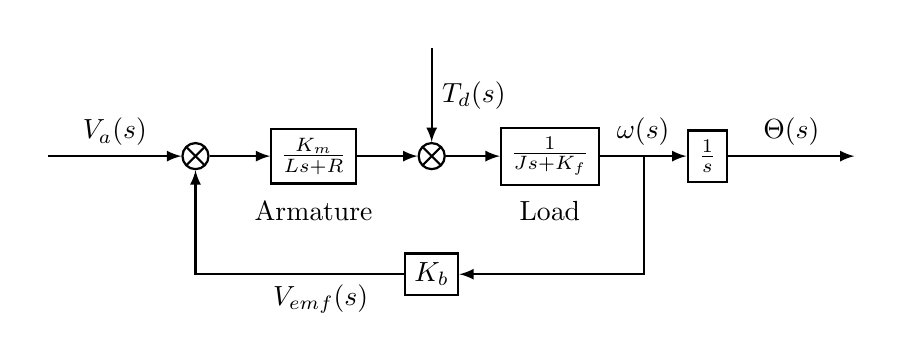
\begin{tikzpicture}[->,use Hobby shortcut,>=latex,thick,node distance = 1.5cm]

\node (start) [startstop] {};
\node (cmp1) [cmppoi,right of=start,xshift=0.5cm] {};
\node (tf1) [tranfun,right of=cmp1,xshift=0cm] {$\frac{K_m}{Ls + R}$};
\node (cmp2) [cmppoi,right of=tf1] {};
\node (tf2) [tranfun,right of=cmp2,xshift=0cm] {$\frac{1}{Js + K_f}$};
\node (tf3) [tranfun,right of=tf2,xshift=0.5cm] {$\frac{1}{s}$};
\node (end) [startstop,right of=tf3,xshift=0.5cm] {};
\node (tf4) [tranfun,below of=cmp2,yshift=0] {$K_b$};
\node (start1) [startstop, above of=cmp2] {};

\node (text1) [startstop, below of=tf1, yshift=0.8cm] {Armature};
\node (text2) [startstop, below of=tf2, yshift=0.8cm] {Load};


\foreach \x in {-0.11,0.11}
{
  \foreach \y in {-0.11,0.11}
  {
    \foreach \i in {1,2}
    {
      \draw[-] (cmp\i.center)--+(\x,\y);
    }
  }
}

\draw (start) -- node[above, pos=0.5]{$V_a(s)$} (cmp1);
\draw (cmp1) -- (tf1);
\draw (tf1) -- (cmp2);
\draw (cmp2) -- (tf2);
\draw (tf2) -- node[above, pos=0.5]{$\omega(s)$} (tf3);
\draw (tf3) -- node[above, pos=0.5]{$\Theta(s)$} (end);
\draw (start1) -- node[right, pos=0.5]{$T_d(s)$} (cmp2);
\draw ($(tf2)+(1.2,0)$) |- (tf4);
\draw (tf4) -| node[below, pos=0.2]{$V_{emf}(s)$} (cmp1);

\end{tikzpicture}



% % new figure
% \begin{tikzpicture}[->, use Hobby shortcut, >=latex, thick, node distance = 1.5cm]

% % startstop 可能表示一个点
% \node (start) [startstop] {};
% \node (cmp) [cmppoi,right of=start,xshift=0.5cm] {};
% \node (tf1) [tranfun,right of=cmp,xshift=0cm] {$D(s)$};
% \node (tf2) [tranfun,right of=tf1,xshift=0cm] {$G(s)$};
% \node (end) [startstop,right of=tf2,xshift=0.5cm] {};

% % 比较器中的斜线
% \foreach \x in {-0.11,0.11}
% {
%   \foreach \y in {-0.11,0.11}
%   {
%     \draw[-] (cmp.center)--+(\x,\y);
%   }
% }

% \draw (start) -- node[above, pos=0.5]{$R(s)$} (cmp) node[above,shift={(-0.2, 0.15)}]{$+$};
% \draw (cmp) -- (tf1);
% \draw (tf1) -- (tf2);
% \draw (tf2) -- node[above, pos=0.5]{$C(s)$} (end);
% \draw ($(tf2)+(1,0)$) -- +(0,-1) -| (cmp) node[below,shift={(0.2,-0.3)}]{$-$};

% \end{tikzpicture}



\end{document}